\documentclass[oneside,11pt]{amsart}
\usepackage[utf8]{inputenc}%
\usepackage[english]{babel}%
\usepackage{amsmath,amssymb,amsthm,amsfonts}%
\usepackage[unicode]{hyperref}%
\usepackage{mathrsfs,bbm}%
\usepackage{paralist}
\usepackage{color}
\usepackage{longtable}
\usepackage{array}
\newcolumntype{L}[1]{>{\small\raggedright\arraybackslash}m{#1}}
\newcolumntype{T}[1]{>{\footnotesize\raggedright\arraybackslash}m{#1}}
\usepackage{stmaryrd}%
%\usepackage{refcheck}
\usepackage{graphicx}
\usepackage[DIV14]{typearea}
\usepackage{multicol,tikz}
\usepackage{datetime}
\usepackage{cleveref}

\usepackage[shadow]{todonotes}

\usepackage{etoolbox}
\patchcmd{\section}{\scshape}{\Large\itshape\bfseries}{}{}

\usepackage{caption}
\captionsetup{labelformat=empty,labelsep=none}

\hypersetup{
  colorlinks=true,
  linkcolor=blue!50!red,
  urlcolor=green!60!black
}

%%%%%%%%%%%%%%%%%%%%%%%%%%%%%%%%%%%%%%%%%%%%%%%%%%%%%%%%%%%%%%%%%%%%%%%%%%%%%%%%%%%%%%%%
\synctex=1
%%%%%%%%%%%%%%%%%%%%%%%%%%%%%%%%%%%%%%%%%%%%%%%%%%%%%%%%%%%%%%%%%%%%%%%%%%%%%%%%%%%%%%%%
%%%%%%%%%%%%%%%%%%%%%%%%%%%%%%%%%%%%%%%%%%%%%%%%%%%%%%%%%%%%%%%%%%%%%%%%%%%%%%%%%%%%%%%%
\newcommand{\score}[1]{\textit{#1}\addtocounter{totalscore}{#1}}
\newcommand{\razdel}[1]{\smallskip\underline{\textbf{#1:}}\smallskip}

\newcommand{\note}[1]{{\sf{}\color{blue}(#1)}}

\begin{document}

\title[MATH 3340: COMPLEX VARIABLES WITH APPLICATIONS]{MATH 3340: COMPLEX VARIABLES WITH APPLICATIONS}
\author{Leonid Petrov\\Spring 2023}
\date{Compiled on \today, \currenttime{}.\\An up to date syllabus is always on \texttt{GitHub} at \url{https://github.com/lenis2000/Syllabi/blob/master/Syllabus_3340_s23.pdf}. For direct PDF download use \href{https://github.com/lenis2000/Syllabi/raw/master/Syllabus_3340_s23.pdf}{\texttt{this link}}.
	\LaTeX{} source with \textit{changes} to the syllabus is \href{https://github.com/lenis2000/Syllabi/blob/master/Syllabus_3340_s23.tex}{\texttt{here}}
(click ``History'').
\\Note that this PDF has green clickable links.}
\maketitle

% \textbf{Important note on registering for the course}: The enrollment deadline is February 1, after five classes have already happened. Before this deadline, two quizzes and two problem set assignments are due, which are a substantial part of the overall course grade. If you are considering taking my class and plan to enroll late, please come to the first classes, even if not officially registered, and submit the coursework --- otherwise, you will miss the credit for these first assignments.

\begin{figure}[h]
	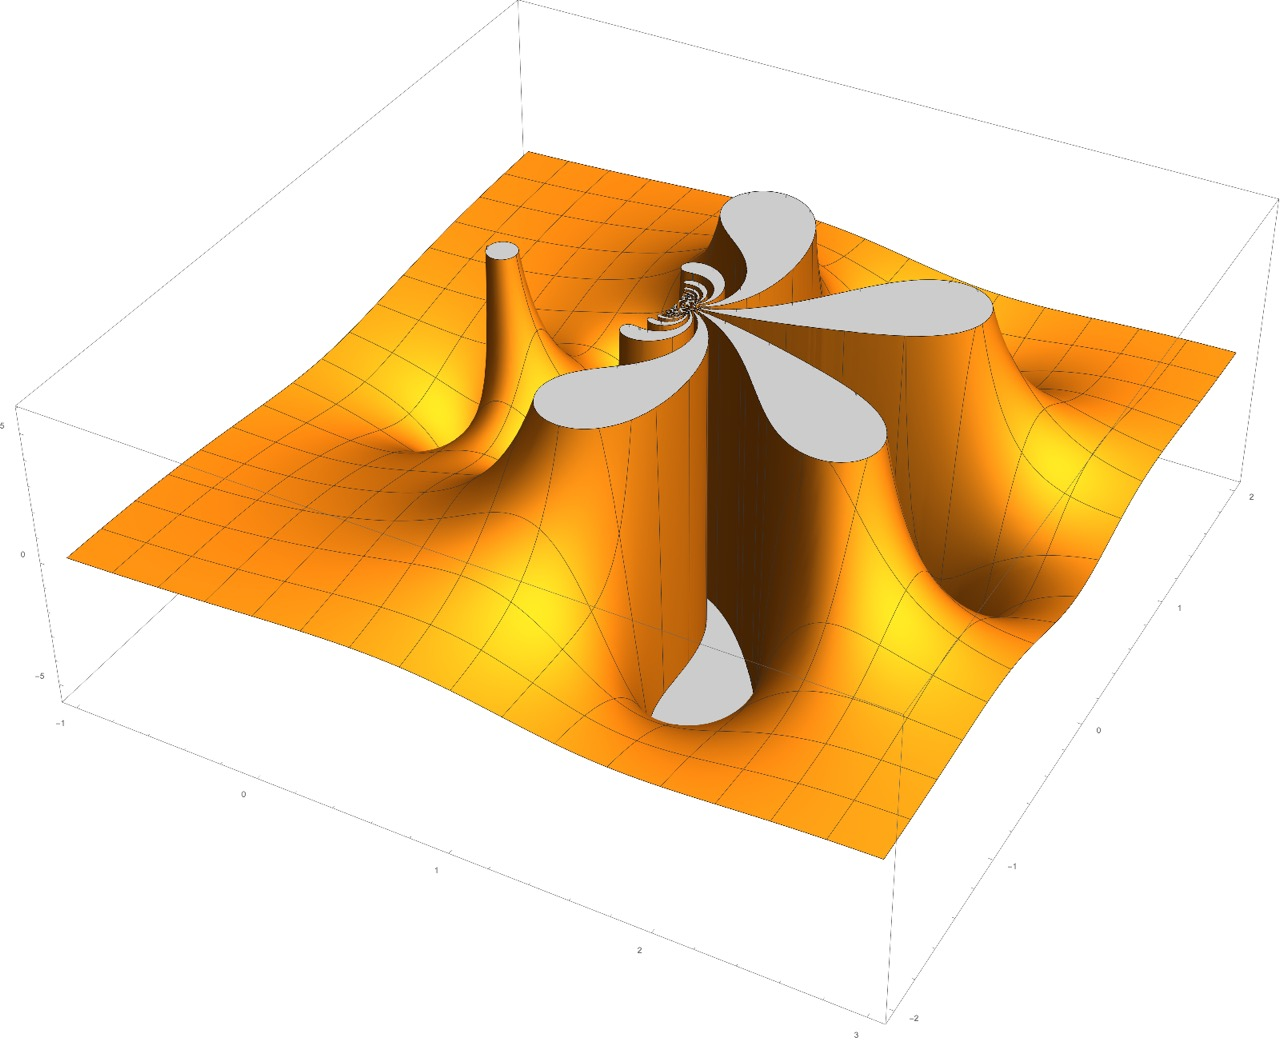
\includegraphics[height=.4\textwidth]{img/complex_f.jpg}
	\qquad 
	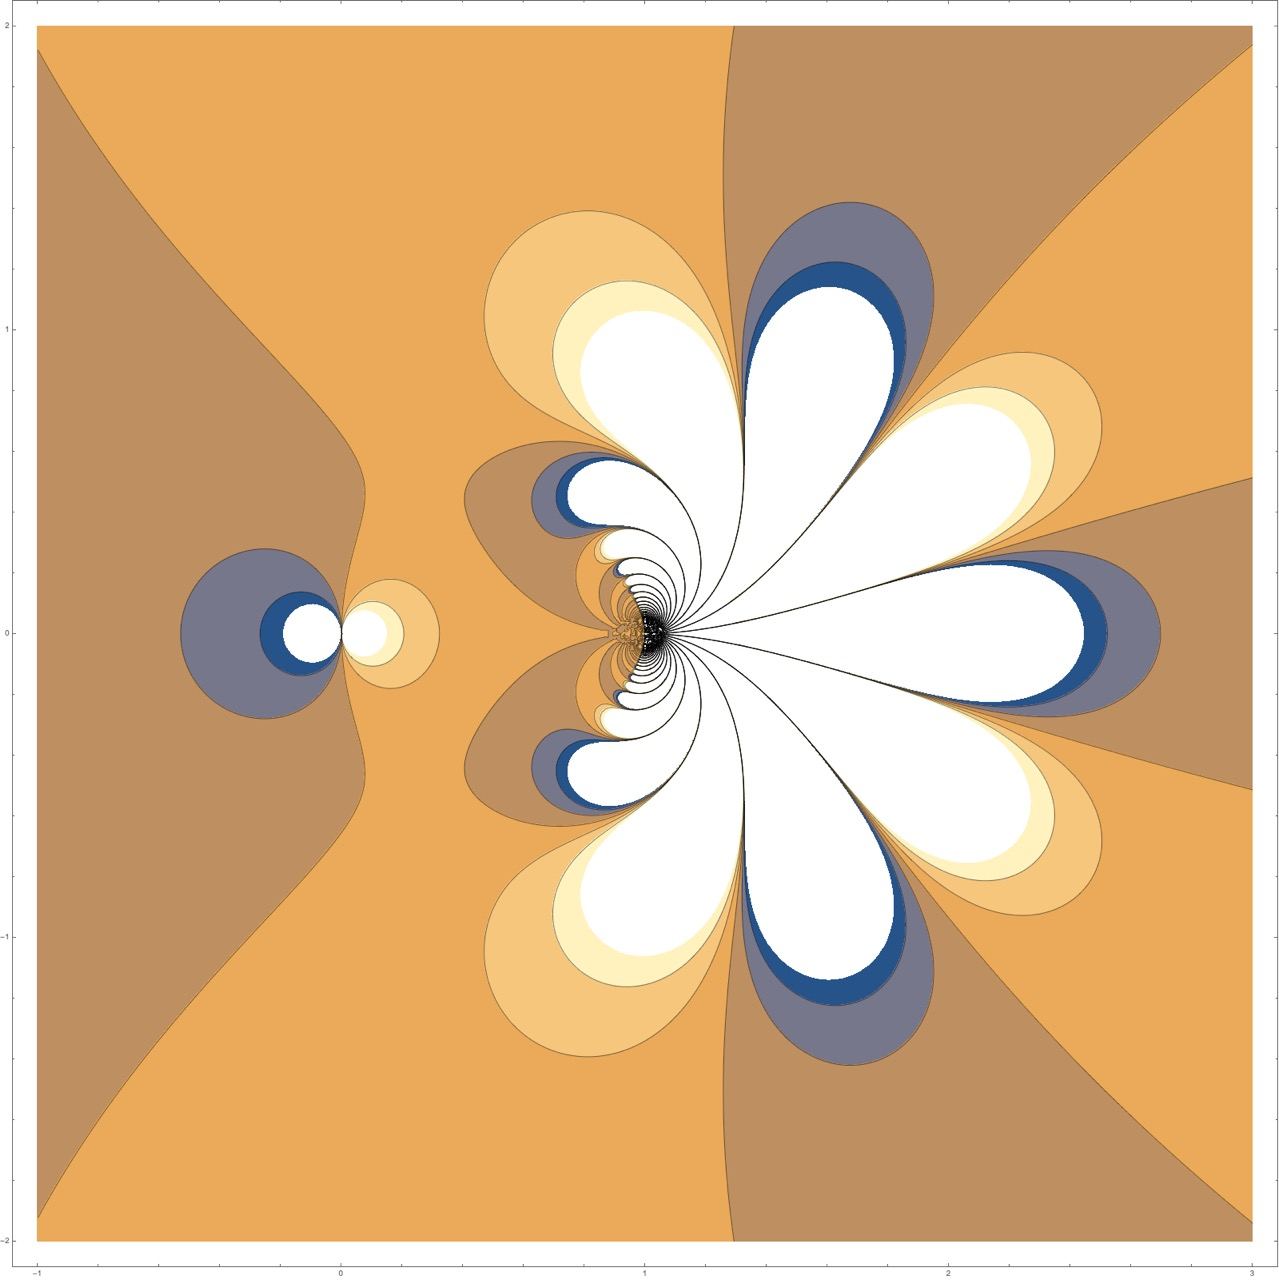
\includegraphics[height=.4\textwidth]{img/complex_f2.jpg}
	\caption{Real part of a particularly complex complex function, and 
	its contour plot on the right.}
\end{figure}

\section{Complex variables}

The course is centered around the theory of functions of a single complex variable and its applications. Complex analysis is a central part of Mathematics. Many concepts work easier and much more naturally in the complex setup:
\begin{itemize}
	\item 
If a function $f(z)$ 
of the complex variable $z$
has one 
derivative at a point $z_0$, then it has infinitely many derivatives,
and possesses a power series (Taylor) expansion at $z_0$, which converges to our function. 
Compare this with the “bad” behavior of the function 
$f(x)=e^{-1/x}$ for $x>0$ (and $f(x)=0$ for $x\le 0$) of the real variable $x$,
which has infinitely many derivatives but whose Taylor series at $0$ is 
identically zero.
\item Any algebraic equation, even $x^{8}+1=0$,
	has a solution over the complex numbers (even
	if no real solutions). In fact, 
	the equation $x^{8}+1=0$ has $8$ different solutions and they all can be 
	illustrated by the vertices of a perfect octagon
	in the complex plane.
\end{itemize}

After taking this course, you 
will be able to solve problems and understand the 
basics of
complex numbers, analytic functions, 
complex integration, Cauchy formulas, power series, 
residues, and conformal mappings.
Moreover, you will learn how to apply these tools to other parts of mathematics and some physical models.

\subsection*{Prerequisites}

Good command of single and multivariable calculus at the level of UVA MATH courses 1310, 1320, and 2310.

\section{Necessary information}
\bigskip

\textbf{Class times:} MoWe 2:00 PM -- 3:15 PM in Monroe 111.

The general structure of each week is (see schedule in \Cref{sec:schedule}):
\begin{itemize}
	\item On Mondays, we have lectures and quizzes. 
	The lectures are recorded and posted to canvas. After the lecture, I may upload an 
	additional recorded piece to canvas if we need the material.
	\item On Wednesdays, we work together in groups to solve homework problems. Homework is due the next Tuesday night.
\end{itemize}

\medskip

\textbf{Exams:}
\begin{itemize}
	\item \textbf{Midterm 1:} Monday, February 13, class time (2:00 PM -- 3:15 PM in Monroe 111)
	\item \textbf{Midterm 2:} Wednesday, April 5, class time (2:00 PM -- 3:15 PM in Monroe 111).
	\item \textbf{Final exam:} Thursday, May 4, 2:00 PM -- 5:00 PM. Monroe 111.
\end{itemize}
Please do not make travel plans that conflict
with the midterms or the final exam. If you have an unavoidable conflict, please notify me as soon as possible.

\medskip

\textbf{Instructor:} Leonid Petrov
\medskip

\textbf{Email:} \email{lenia.petrov+s23@gmail.com} (preferred)
\medskip

\textbf{Office:} 209 Kerchof Hall
\medskip

\textbf{Office hours:}
Mondays 12PM -- 1PM (Kerchof 209) and Tuesdays 1PM -- 2PM (on Zoom), starting on January 23.

Zoom link for office hours is available on Canvas.

\medskip

You are welcome to make an appointment and meet with me on Zoom outside the usual office hours
or this, please use the online tool located at
\url{https://lpetrov.cc/teaching/}. (I am automatically available during office hours --- 
and you cannot schedule appointments online for those times.)
You can make as 
many extra appointments as you want.

\medskip

\textbf{Course webpage:}
We will use the Canvas course page for problem set submissions, course materials, recorded 
lectures, and communication. We will use Canvas discussions as a public space to ask and answer questions. 
\textit{Please keep the Canvas notifications on for announcements.}
The Canvas mobile App is also useful for quick course communication.

\section{Course materials}
\label{sec:textbook}

Note: it is not required to purchase a textbook to succeed in the course.

\medskip

\textbf{Main textbook:}
\emph{Complex Analysis a First Course with Applications} (third edition)
by
Zill, Dennis G. and Shanahan, Patrick D. 
ISBN: 9781449694616

\medskip


Optional textbook: “\emph{Fundamentals of Complex Analysis}” (3rd edition)
by Saff and Snider, Pearson, ISBN-10: 0139078746.
% We will discuss material from Chapters 1--6, and selected topics from Chapters 7--8.

\medskip

In addition, there is a number of online resources which may help you while doing the homework:
Khan Academy, Wikipedia, YouTube, and many other 
places contain lots of basic material on complex analysis. 
For example, check out this video by 3blue1brown: \url{https://www.youtube.com/watch?v=5PcpBw5Hbwo}.
Google Search
in general
is also a valuable resource.

\section{Assessing your learning}

\subsection*{Overview}

The general structure of each week is (see schedule in \Cref{sec:schedule}):
\begin{itemize}
	\item On Mondays, we have lectures and quizzes. 
	The lectures are recorded and posted to canvas. After the lecture, I may upload an 
	additional recorded piece to canvas if we need the material.
	\item On Wednesdays, we work together in groups to solve homework problems. Problem set is due the next Tuesday night.
\end{itemize}
For example, on Monday 3/20 we have a lecture and a quiz. The quiz is based on the previous two weeks' material. 
On Tuesday 3/21 the problem set discussed on Wednesday 3/15 is due.
On Wednesday 3/22, we start discussing a new problem set which is due on 3/28.

\medskip

Learning mathematics means \emph{doing} mathematics: during class meetings, on your own, and in groups. 
In this course, doing mathematics mainly amounts to solving problems.
Below are the concrete aspects which are assessed in this course:

\subsection{Homework (20\%)}

The homework has two parts:
\begin{enumerate}
	\item By each Wednesday when we start a new problem set, 
		you should review the previous lecture material, including a possible
		extra recorded piece.
	\item Problem sets are due on Tuesdays to Canvas. Each new problem sets begins with a group discussion
		on Wednesday the previous week.
\end{enumerate}

Putting an adequate effort into solving the homework
problems and
communicating your solutions clearly is
of paramount importance for your learning.

The problem sets are graded ``coarsely'', that is,
each homework will be assigned one of four grades: 
\begin{equation*}
\begin{tabular}{l|l|l|l|l}
Grade & VG (very good) & G (good) & OK   & N \\
\hline
& \parbox{.21\textwidth}{All problems solved correctly with minor issues like arithmetic mistakes, and solutions explained
in full detail}
& \parbox{.21\textwidth}{Most problems solved correctly, and solutions explained in reasonable (close to full) detail}
& \parbox{.21\textwidth}{ {\ }\\More than $3/4$ of problems attempted, many 
solutions are incorrect, incomplete, or not explained in detail, 
but the work displays adequate understanding of most of the material\\{}}
& \parbox{.21\textwidth}{Work not submitted on time, or less than $3/4$ of problems 
attempted, or most solutions are incomplete, or work clearly displays lack of understanding of most of the material}\\
\hline
\%    & 100\%          & 90\%     & 75\% & 0\%
\end{tabular}
\end{equation*}
It is expected that most students 
who put reasonable effort into the homework
will get VG or G grades. 

There are 11 regular problem sets out of which 2 lowest will be dropped.
On May 2, there is an extra opportunity to repair your course credit (only if it is low)
by submitting an extra problem set (or solving optional exercises from the previous problem sets --- this is to be decided as we go).

\subsection*{Homework submission guidelines --- strictly enforced}
The homework \textbf{must be submitted only on Canvas} (i.e., hard copies are not accepted).
Take pictures or scan your work,
make sure it's readable,
put it into a \emph{single PDF file with correct orientation},
and upload it before the deadline.

Submitting work like this has many benefits:
(1) you retain a paper copy to
prepare for tests;
(2) your submitted work is never misplaced or lost, and there is a digital trail;
(3) the grading will be faster.
If you have any trouble submitting homework online, ask me for help.

\subsection*{Note on collaboration on homework assignments}
\label{collaboration}

Group work on homework problems is allowed and encouraged.
Discussions are in general very
helpful and inspiring when learning mathematics.
The work on each problem set will start with an in-class group discussion.

However, when completing the written homework assignments, everyone must write up their own
solutions in their own words.
It is very important that you truly understand the homework solutions you hand
in, otherwise you may be unpleasantly surprised by your in-class test results.

When working on in-class assignments (quizzes, tests)
you are required to work alone.

\subsection{Quizzes (20\%)}

There will be short quizzes (20min) on Mondays after the lecture.
The quiz problems are based on the class material from the previous two weeks
and/or recent homework topics.

Quizzes are open notes, but no collaboration allowed.
Quizzes test your ``work in progress'', and also make sure that you are regularly present at lectures.

We have 11 quizzes planned, 2 lowest will be dropped. If snowstorms remove more than two Mondays, 
we will adjust and drop 1.5 lowest quizzes out of 9.

\subsection{Midterm tests (13\% each) and the final exam (24\%)}

The midterms and the final exam will feature
problems modeled after homework/quizzes.
The final exam is comprehensive, with a focus on the last part
after the second midterm.

The exams will be aimed at checking not so much memorization and
routine computational skills, but rather understanding of fundamental
concepts and principles and the ability to apply the material
learned to solving various problems, including those a student might
have never seen before. A missed exam gives a score of zero, unless a
student has contacted the instructor a week in advance and agreed upon a
procedure to make it up. Under the rules of
the College, early examinations are not permitted.

\medskip

A two-sided letter size formula sheet, hand-written by yourself, is
allowed on each midterm test and on the final exam.
(Other than this, no notes allowed.)
Preparing this formula sheet
will help you review the material, and paint a systematic picture of the material in your mind.
In general, formula sheets cannot contain any photocopied or
printed material --- do everything by hand (of course, you can
include any theorems, formulas, pictures, examples, etc).
One exclusion: if you write the formula sheet out on a
tablet and print, this is allowed, if helps --- but don't copy
formula sheets from other people.

I encourage you to collaborate on preparing for the tests, but needless to say that
during the test and the final exam each student must work individually.

\subsection*{How to succeed in the course}

The best way to learn in the course is to come to all lectures and watch the extra recorded pieces, take good notes,
ask many questions,
do all the homework problems, and express your solutions
clearly.
This will prepare you well for quizzes, midterms, and the final exam.

Mathematical questions are appreciated and encouraged any time during the
class. Please use the office hours as much as possible for additional
clarifications and occasional homework help. Remember that I am available outside 
of office hours by appointment which you can book at
\url{https://lpetrov.cc/teaching/}

\subsection{Grade distribution}

Your grade will consist of:
\begin{itemize}
	\item Homework --- 20\% (2 lowest dropped)
	\item Quizzes --- 20\% (2 lowest dropped)
	\item Two midterms --- 13\% each
	\item Final exam --- 24\%
	\item Class participation, office hours discussion --- 10\%
\end{itemize}
If by late April your course grade is low, there is an opportunity to submit an extra
``repair credit'' assignment (to be decided exactly as we go). This assignment will not 
increase an already good grade, but will only improve a not so good one.

The scale by which course percent grades are turned into course letter grades
will most likely be the following:
\begin{equation*}
	\begin{tabular}{l|l|l|l|l|l|l|l|l|l|l|l|l|}
		Grade      & $ A+	$ & $A	$ & $A-	$ & $B+	$ & $B	$ & $B-	$ & $C+	$ & $C	$ & $C-	$ & $D+	$ & $D	$ & $D-$ \\
		\hline
		Minimum \% & 100     & 93   & 89    & 86    & 82    & 79    & 76    & 72    & 69    & 66    & 62    & 59
	\end{tabular}
\end{equation*}
I reserve the right to slightly change this grade scale after the
final exam.
This may be needed
to better incorporate into the letter grade
possible fluctuations in the difficulty level of 
midterms and the final.

\section{Course schedule (updated as we go)}
\label{sec:schedule}

Sections are from the Zill--Shanahan textbook.

\begin{enumerate}[\bf{}{[}week 1{]}]
	\item 1/18. Algebra and geometry of complex numbers (1.1--1.2).
	\item 1/23[Q1], 1/25. Problem set 1 due 1/24, 10pm.\footnote{All assignments are due at 10 pm instead of midnight because of the common need to sleep.}
		Polar coordinates. Subsets of the complex plane: open, close, connected, domains, bounded, etc (1.3, 1.5).
	\item 1/30[Q2], 2/1. Problem set 2 due 1/31, 10pm.
		Complex plane and Riemann sphere (1.5).
		Elementary complex functions: exponential, powers and roots (1.4, 1.6).
		Complex functions (2.1).
	\item 2/6[Q3], 2/8. Problem set 3 due 2/7, 10pm.
		Mappings of the complex plane: linear, powers and roots, 1/z (chapter 2).
	\item \textbf{2/13}[M1], 2/15.
		Limits, continuity, derivatives
		(2.6, 3.1).
	\item 2/20[Q4], 2/22. Problem set 4 due 2/21, 10pm.
		Complex derivative and analyticity. Cauchy-Riemann equations.  Harmonic functions.
		(3.1, 3.2, 3.3)

		\colorbox{yellow}{\parbox{.7\textwidth}{we are here}}
	\item 2/27[Q5], 3/1. Problem set 5 due 2/28, 10pm.
	\item 3/13[Q6], 3/15. Problem set 6 due 3/14, 10pm.
	\item 3/20[Q7], 3/22. Problem set 7 due 3/21, 10pm.
	\item 3/27[Q8], 3/29. Problem set 8 due 3/28, 10pm.
	\item 4/3, \textbf{4/5}[M2].
	\item 4/10, 4/12. Problem set 9 due 4/11, 10pm.
	\item 4/17[Q9], 4/19. Problem set 10 due 4/18, 10pm.
	\item 4/24[Q10], 4/26. Problem set 11 due 4/25, 10pm.
	\item 5/1[Q11]. Repair credit problem set 12 due 5/2, 10pm.
\end{enumerate}

\medskip

[Q]: quiz, [M]: midterm.

\section{Policies}

\subsection{Late/make up work} 

Each homework assignment will have a due date and time by which it must be submitted to Canvas.  After the 1-hour grace period, late assignments are not accepted.  There will also be no make-up for the quizzes or midterm tests.  However, if you have special needs, emergencies, or unavoidable conflicts, please let me know as soon as possible so we can arrange a workaround for the midterms and the final exam.

\subsection{Special needs}

All students with special needs requiring accommodations should present the appropriate paperwork from the Student Disability Access Center (SDAC). The student must present this paperwork in a timely fashion and follow up with the instructor about the accommodations being offered.  Accommodations for midterms or final exams (e.g., extended time) should be arranged (booked with SDAC) at least five days before an exam.

\subsection{Honor Code} 

The University of Virginia Honor Code applies to this class and is taken seriously (in particular, see \Cref{collaboration} on homework collaboration).  Any honor code violations, especially in written tests (midterms and the final exam), will be referred to the Honor Committee.


\end{document}
